% 本文件是由赵启所撰写的“软件分析”章节中的有限元部分抽离出来的
% 修改者:谭正
% 上次更新:2020年1月14日12点03分

\subsection{云台主轴的有限元分析}

在对云台主轴进行有限元分析之前,需要进行前处理:输入蜗杆的几何模型、对几何模型划分网格。并根轴的实际受力情况施加载荷(图~\ref{fig:shaft_load},A处受到蜗轮输出的扭矩和蜗轮的重力;B处受到大臂向下压轴的径向力,姑且假定两边对称;D和E分别是四个径向约束和两个扭转约束。)求解后进行输出应力应变云图。

  \begin{figure}[!h]
    \centering
    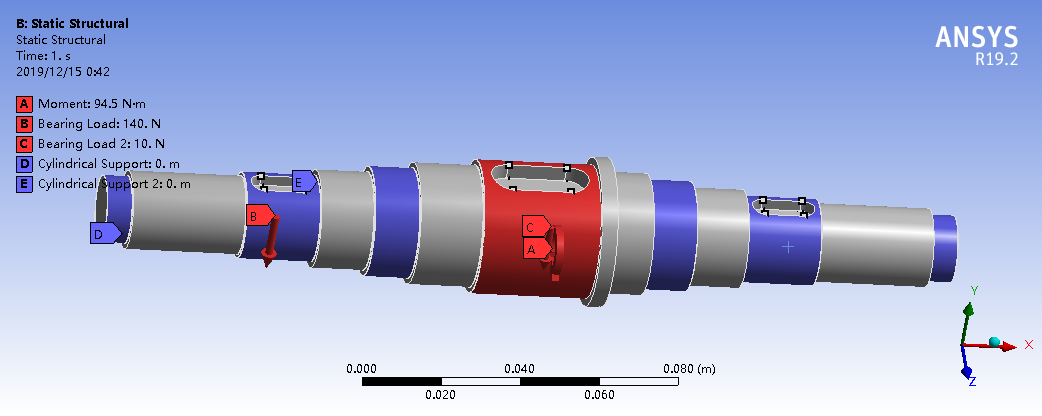
\includegraphics[width=12cm]{stress_and_torque_of_worm.png}
    \bicaption[云台主轴所受载荷和约束情况]{云台主轴所受载荷和约束情况}{Loads and constraints on the gimbal spindle}
    \label{fig:shaft_load}
  \end{figure}

  从图~\ref{fig:normalStress}、图~\ref{fig:shearStress}和图~\ref{fig:tensiledis}中可以清楚地看到:按云台主轴原本所设计的尺寸计算,正应力,拉伸位移都在许用值以内,只是有一小部分的剪切应力超出了许用值,但考虑到实际工作中满载的几率微乎其微,对轴的实际使用寿命影响很小,也考虑到经费的原因,故决定不再加粗,就以此尺寸加工。

  \begin{figure}[!htp]
    \centering
    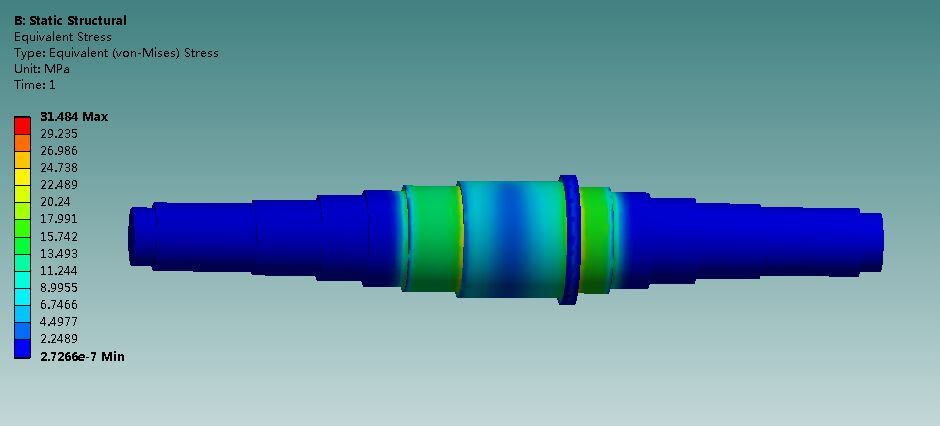
\includegraphics[width=12cm]{normal_stress.jpg}
    \bicaption[云台主轴的正应力云图]{正应力}{Normal stress}
    \label{fig:normalStress}
  \end{figure}

  \begin{figure}[!htp]
    \centering
    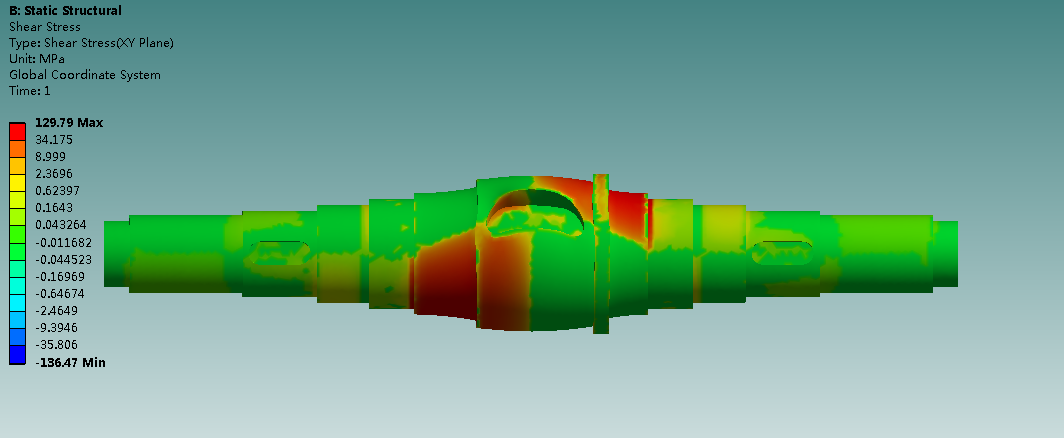
\includegraphics[width=12cm]{shear_stress.png}
    \bicaption[云台主轴的切应力云图]{切应力}{Shear stress}
    \label{fig:shearStress}
  \end{figure}

  \begin{figure}[!htp]
    \centering
    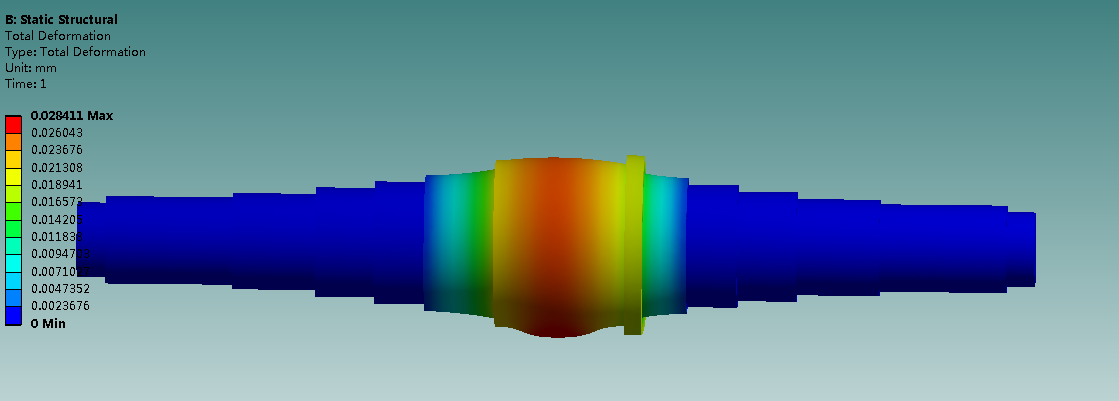
\includegraphics[width=12cm]{tensile_displacement.png}
    \bicaption[云台主轴的拉伸位移云图]{拉伸位移}{Tensile displacement}
    \label{fig:tensiledis}
  \end{figure}
